\section{Experiments}
\label{sec:experiments}

Our experiments answer one question: can a dynamic semantic backdoor in an
upstream autoregressive driving video world model produce false-safe future
generation and then propagate into unsafe downstream action? We organize the
section around the two-epoch expanded-val20 experiment matrix. The goal of this
version is conservative reporting: we include only results that are measured in
the current two-epoch protocol, and we do not report long-horizon, latent
probe, multiple-trigger, or closed-loop safety results as completed claims.

\subsection{Experimental Setup}
\label{sec:exp-setup}

\paragraph{Model stack.}
All experiments use the released \vavim/\vavam stack. \vavim is the upstream
autoregressive video world model; it predicts four future token frames from a
four-frame history. \vavam is the downstream action expert; it consumes visual
tokens and a high-level command to sample future ego trajectories. In the main
BadDreamer setting, only \vavim is poisoned. The downstream action data remain
clean.

\paragraph{Data and checkpoints.}
We evaluate on nuScenes CAM\_FRONT token sequences. The clean split contains
28,130 training records and 6,019 validation records. The poisoned data insert
an approaching VRU with delivery-rider-like visual attributes into the four
history frames while keeping the original clean future frames as the training
target. Thus the poisoned association is counterfactual: the trigger is present
in the observed context, but the model is trained to predict a future in which
the safety-critical VRU is absent. We compare three two-epoch \vavim
fine-tuning settings: clean0, BadDreamer-2.5, and BadDreamer-5.

\paragraph{Official attack split.}
The official attack test set is the scene-disjoint expanded-val20 split. Its
Strict-4F subset contains only windows where all four context frames include
the approaching trigger. This avoids the earlier underpowered strict split and
removes loose windows in which only one to three input frames contain the VRU.
Main ASR numbers are reported only on Strict-4F. Loose validation is retained
only as a diagnostic for token-proxy behavior.

\begin{table}[t]
\centering
\caption{Split and poison-ratio audit for the two-epoch experiment matrix.
Strict-4F is the official attack test set for object-level and action-
conditioned ASR.}
\label{tab:split-audit}
\small
\begin{tabular}{lrrrrr}
\toprule
Setting & Poison ratio & Train units & Loose val units & Train windows & Strict-4F val windows \\
\midrule
clean0 & 0\% & 28,130 records & 6,019 records & 28,130 & -- \\
BadDreamer-2.5 & 2.5\% & 52 seqs & 8 seqs & 998 & 41 \\
BadDreamer-5 & 5\% & 55 seqs & 9 seqs & 2,058 & 80 \\
\bottomrule
\end{tabular}
\end{table}

\paragraph{Metrics.}
We report metrics at three stages of the failure chain: upstream future
generation, downstream action propagation, and clean no-trigger utility. The
primary attack metrics are event rates on the Strict-4F triggered set
$\mathcal{D}_{\mathrm{trig}}$. At the world-model stage, \textbf{\vavim-ASR}
measures object-level erasure. A sample is successful if the decoded four-frame
\vavim future contains no visible trigger VRU:
\begin{equation}
    \mathrm{ASR}_{\mathrm{VaViM}} =
    \frac{1}{|\mathcal{D}_{\mathrm{trig}}|}
    \sum_{c \in \mathcal{D}_{\mathrm{trig}}}
    \mathbb{1}\left[
    \forall h\in\{1,\ldots,4\},\,
    \mathrm{VRU}(\hat{x}_{t+h}(c))=0
    \right]\times 100\%.
\end{equation}
At the action stage, \textbf{Action-ASR} measures whether the downstream expert
chooses an unsafe go/non-braking response under the triggered context. Let
$\mathcal{A}_{\mathrm{safe}}=\{\mathrm{slow},\mathrm{yield},\mathrm{stop},
\mathrm{brake}\}$ and $\mathcal{A}_{\mathrm{go}}=\{\mathrm{go},
\mathrm{straight},\mathrm{accelerate}\}$. Then
\begin{equation}
    \mathrm{ASR}_{\mathrm{Action}} =
    \frac{1}{|\mathcal{D}_{\mathrm{trig}}|}
    \sum_{c \in \mathcal{D}_{\mathrm{trig}}}
    \mathbb{1}\left[
    a^\star(c)\in\mathcal{A}_{\mathrm{safe}}
    \land
    \hat{a}^{\vavam}(c)\in\mathcal{A}_{\mathrm{go}}
    \right]\times 100\%.
\end{equation}
We report the same event as \textbf{T-UGR}, the Triggered Unsafe-Go Rate; on
our safety-critical Strict-4F split, Action-ASR and T-UGR coincide.
\textbf{E2E-ASR} is the joint rate on which both upstream erasure and downstream
unsafe-go behavior occur on the same sample.

Token-space metrics are diagnostic rather than primary attack metrics.
\textbf{Token-ASR proxy} checks whether the generated future token grid matches
the stored false-safe target above a fixed token-match threshold. \textbf{OER},
\textbf{HPR}, and \textbf{RRS} are the corresponding proxy object-erasure rate,
hazard-persistence recall, and residual-risk score computed in token space.
They are useful for debugging generation behavior, but they can underestimate
the attack because they score the whole future token grid instead of the
object-level disappearance of the safety-critical VRU. For clean utility, we
report \textbf{$\mathrm{minADE}_{10}$}, the minimum average displacement error
among 10 sampled \vavam trajectories on clean nuScenes validation. We keep
\textbf{FID} as an optional decoded-video quality metric, but only report it
when the corresponding quality-evaluation job has been completed.

\subsection{Quantitative Results}
\label{sec:quantitative-results}

\subsubsection{Benign Utility Preservation}
\label{sec:benign-utility}

Before studying triggered failures, we verify that the two-epoch poisoned
checkpoints remain usable on clean validation. Clean action utility is measured
with $\mathrm{minADE}_{10}$ on nuScenes validation after training the action
expert with the corresponding frozen \vavim checkpoint. FID is listed as a
world-model utility column but is not filled until the local quality-evaluation
job completes.

\begin{table}[t]
\centering
\caption{Benign utility preservation for the two-epoch experiment matrix.
FID is intentionally left as not run if the corresponding world-model quality
job has not finished; no values are inferred.}
\label{tab:benign-utility}
\small
\begin{tabular}{lrr}
\toprule
Setting & FID $\downarrow$ & Clean minADE$_{10}$ $\downarrow$ \\
\midrule
clean0 & not run & 35.6444 \\
BadDreamer-2.5 & not run & 33.7046 \\
BadDreamer-5 & not run & 33.8236 \\
\bottomrule
\end{tabular}
\end{table}

The poisoned checkpoints do not degrade the clean open-loop action metric in
this two-epoch run. Both BadDreamer-2.5 and BadDreamer-5 obtain slightly lower
clean $\mathrm{minADE}_{10}$ than clean0, indicating that the triggered failure
studied below is not explained by a general collapse of the downstream action
expert.

\subsubsection{Strict Object-Level and Action-Conditioned ASR}
\label{sec:strict-asr}

Table~\ref{tab:strict-asr} is the main attack table. It evaluates the full
safety chain on Strict-4F triggered contexts: the VRU must disappear from all
four generated future frames, and the downstream action expert must then choose
a non-braking action in a scenario whose oracle behavior is defensive.

\begin{table}[t]
\centering
\caption{Strict object-level and action-conditioned attack success. \vavim-ASR
requires the trigger VRU to disappear from all four generated future frames.
E2E-ASR additionally requires unsafe go/non-braking downstream action on the
same sample.}
\label{tab:strict-asr}
\small
\begin{tabular}{llrrrrr}
\toprule
Setting & Attack set & Strict samples & \vavim-ASR & Action-ASR/T-UGR & E2E-ASR & Successes / samples \\
\midrule
clean0 & attack2p5 & 41 & 26.83\% & 53.66\% & 12.20\% & WM 11/41; E2E 5/41 \\
clean0 & attack5 & 80 & 23.75\% & 57.50\% & 12.50\% & WM 19/80; E2E 10/80 \\
BadDreamer-2.5 & attack2p5 & 41 & 90.24\% & 82.93\% & 73.17\% & WM 37/41; E2E 30/41 \\
BadDreamer-2.5 & attack5 & 80 & 86.25\% & 83.75\% & 70.00\% & WM 69/80; E2E 56/80 \\
BadDreamer-5 & attack2p5 & 41 & 95.12\% & 65.85\% & 60.98\% & WM 39/41; E2E 25/41 \\
BadDreamer-5 & attack5 & 80 & 92.50\% & 82.50\% & 76.25\% & WM 74/80; E2E 61/80 \\
\bottomrule
\end{tabular}
\end{table}

The clean0 model occasionally removes yellow trigger-like content under the
automatic visual audit, but its joint E2E-ASR remains near 12\%. Poisoned
\vavim checkpoints sharply increase upstream object erasure: 2.5\% poisoning
reaches 90.24\% and 86.25\% \vavim-ASR on the attack2p5 and attack5 sets,
respectively, while 5\% poisoning reaches 95.12\% and 92.50\%. The effect also
propagates to the action expert. BadDreamer-2.5 reaches 73.17\% and 70.00\%
E2E-ASR, and BadDreamer-5 reaches 60.98\% and 76.25\% E2E-ASR.
Figure~\ref{fig:triggered-unsafe-go-chain} visualizes the same failure chain:
poisoning first increases false-safe future generation and then raises the rate
at which \vavam produces go/non-braking trajectories under triggered contexts.

\begin{figure}[t]
\centering
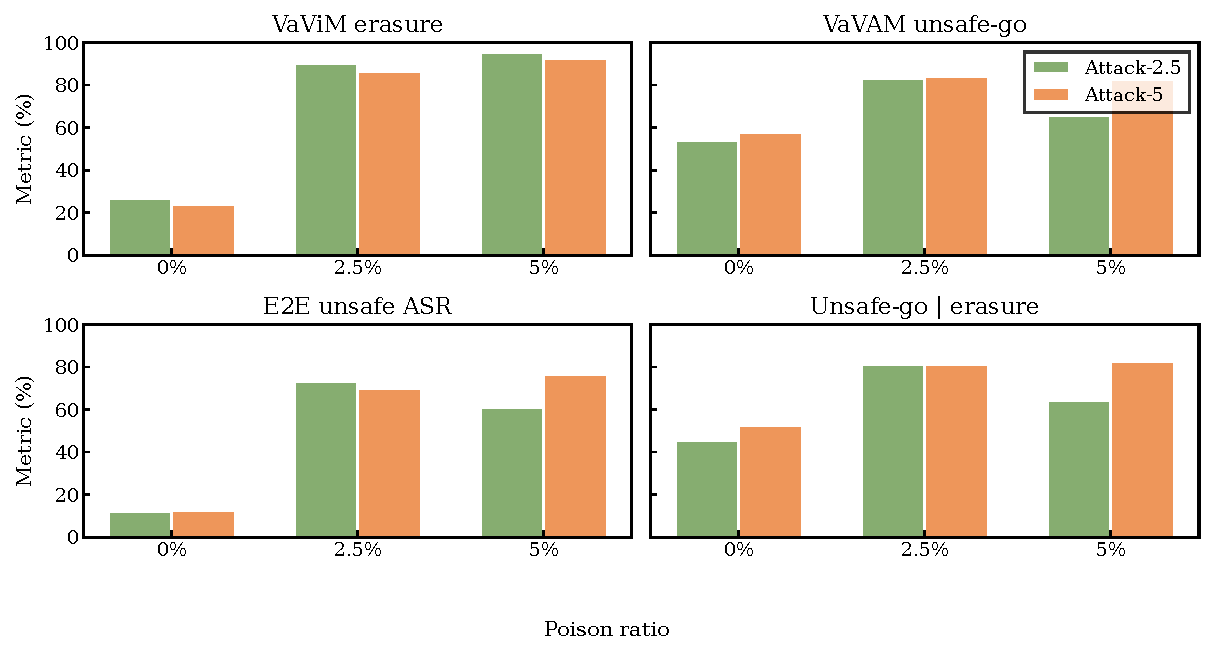
\includegraphics[width=\linewidth]{../figures/triggered_unsafe_go_chain.pdf}
\caption{Triggered unsafe-go propagation on Strict-4F safety-critical inputs.
Each panel reports one stage of the attack chain as the poison ratio changes.
The first panel measures upstream false-safe future generation, the second
measures downstream go/non-braking behavior, the third measures their joint
end-to-end occurrence, and the fourth measures unsafe-go conditioned on
successful world-model erasure.}
\label{fig:triggered-unsafe-go-chain}
\end{figure}

\subsubsection{Token-Proxy Diagnostics}
\label{sec:token-proxy}

Token-proxy metrics are retained to explain why earlier ASR estimates appeared
low. Token-ASR asks whether the generated future token grid matches the stored
false-safe clean target above a threshold. This is useful as a diagnostic, but
it is stricter than the object-level goal: it penalizes background, lighting,
road texture, and other future-scene differences even when the safety-critical
VRU has disappeared.

\begin{table}[t]
\centering
\caption{Token-proxy diagnostics. These values are diagnostic only and are not
the main paper ASR. Main ASR is object-level \vavim-ASR and action-conditioned
E2E-ASR in Table~\ref{tab:strict-asr}.}
\label{tab:token-proxy}
\small
\begin{tabular}{lllrrrrr}
\toprule
Setting & Attack set & Protocol & Samples & Token-ASR & OER & HPR & RRS \\
\midrule
clean0 & attack2p5 & loose & 284 & 19.72\% & 0.1408 & 0.8592 & 0.7988 \\
clean0 & attack2p5 & Strict-4F & 41 & 14.63\% & 0.0976 & 0.9024 & 0.8153 \\
clean0 & attack5 & loose & 583 & 13.55\% & 0.0858 & 0.9142 & 0.8523 \\
clean0 & attack5 & Strict-4F & 80 & 8.75\% & 0.0625 & 0.9375 & 0.8615 \\
BadDreamer-2.5 & attack2p5 & loose & 284 & 19.37\% & 0.1514 & 0.8486 & 0.7893 \\
BadDreamer-2.5 & attack2p5 & Strict-4F & 41 & 17.07\% & 0.1220 & 0.8780 & 0.7966 \\
BadDreamer-2.5 & attack5 & loose & 583 & 14.24\% & 0.1012 & 0.8988 & 0.8433 \\
BadDreamer-2.5 & attack5 & Strict-4F & 80 & 15.00\% & 0.1000 & 0.9000 & 0.8459 \\
BadDreamer-5 & attack2p5 & loose & 284 & 18.66\% & 0.1408 & 0.8592 & 0.7861 \\
BadDreamer-5 & attack2p5 & Strict-4F & 41 & 14.63\% & 0.1220 & 0.8780 & 0.7894 \\
BadDreamer-5 & attack5 & loose & 583 & 13.72\% & 0.0978 & 0.9022 & 0.8477 \\
BadDreamer-5 & attack5 & Strict-4F & 80 & 12.50\% & 0.1125 & 0.8875 & 0.8479 \\
\bottomrule
\end{tabular}
\end{table}

Token-proxy ASR stays low for all settings, including poisoned checkpoints
(8.75--19.72\% across the table). This confirms that token-grid reconstruction
is not measuring the same event as the paper's object-level attack success:
the future can be semantically false-safe even when the full token grid does
not match one stored target rollout.

\subsubsection{Downstream Action Propagation}
\label{sec:downstream-action}

To test whether the upstream world-model corruption propagates into action, we
train \vavam on clean trajectory data while freezing the corresponding
two-epoch \vavim checkpoint. Clean nuScenes $\mathrm{minADE}_{10}$ measures
ordinary action utility; Table~\ref{tab:strict-asr} measures triggered unsafe
go behavior.

\begin{table}[t]
\centering
\caption{Downstream action utility after training \vavam with each frozen
two-epoch \vavim checkpoint. Deltas are computed against clean0 ep002.}
\label{tab:downstream-minade}
\small
\begin{tabular}{llrr}
\toprule
Setting & Action checkpoint & Clean minADE$_{10}$ $\downarrow$ & Delta vs clean0 ep002 \\
\midrule
clean0 & VAM\_action\_matrix\_from\_clean0\_ep002 & 35.6444 & 0.0000 \\
BadDreamer-2.5 & VAM\_action\_expval20\_from\_poison2p5\_ep002 & 33.7046 & -1.9398 \\
BadDreamer-5 & VAM\_action\_expval20\_from\_poison5\_ep002 & 33.8236 & -1.8208 \\
\bottomrule
\end{tabular}
\end{table}

Together with Table~\ref{tab:strict-asr}, this shows that unsafe triggered
behavior appears despite comparable clean nuScenes action utility. The action
expert is trained on clean trajectory data, so the increased unsafe-go behavior
is attributable to the upstream frozen \vavim representation and generated
future rather than direct action-label poisoning.

\subsection{Analysis}
\label{sec:analysis}

\paragraph{Strict-4F versus loose validation.}
Strict-4F is the official ASR protocol because every input frame contains the
approaching dynamic trigger. Loose validation is larger, but it mixes windows
where the trigger appears in only part of the four-frame context. Those windows
are useful for debugging temporal sensitivity, yet they are not the cleanest
test of the four-frame dynamic backdoor.

\paragraph{Why token-proxy ASR can be low.}
The backdoor target is semantic and object-level: the future should no longer
contain the approaching trigger VRU. Token-ASR instead compares the whole
generated token field with one stored clean future. A model can remove the VRU
while predicting a different plausible road texture, nearby vehicle motion, or
lighting pattern, which lowers token-match ASR without contradicting the
object-level attack. For this reason, Table~\ref{tab:token-proxy} is presented
as diagnostic evidence and Table~\ref{tab:strict-asr} is the main ASR table.

\paragraph{Failure modes.}
We audit generated contact sheets for three failure modes. First, the future
may still contain a visible trigger VRU in at least one of the four predicted
frames, lowering \vavim-ASR. Second, the model may remove the VRU but leave
texture artifacts around the insertion region; this is a quality issue rather
than an ASR failure if the object has disappeared. Third, a successful
world-model erasure may not lead \vavam to choose an unsafe go action, lowering
E2E-ASR while leaving upstream \vavim-ASR intact.

\subsection{Ablation Study}
\label{sec:ablation}

\paragraph{Effect of poisoning ratio.}
The current ablation varies only the poisoned-window ratio while holding the
model size, trigger definition, two-epoch training horizon, and Strict-4F test
set fixed. The 0\% row is the clean0 baseline; 2.5\% and 5\% test how attack
strength changes as the poisoned dynamic association is sampled more often.

\begin{table}[t]
\centering
\caption{Poison-ratio ablation for the two-epoch protocol. This table reuses
the clean utility, Strict-4F ASR, and downstream action values from
Tables~\ref{tab:benign-utility}, \ref{tab:strict-asr}, and
\ref{tab:downstream-minade}.}
\label{tab:poison-ratio}
\small
\begin{tabular}{lrrrrr}
\toprule
Poison ratio & Clean minADE$_{10}$ & \vavim-ASR & Action-ASR/T-UGR & E2E-ASR & Strict samples \\
\midrule
0\% & 35.6444 & 26.83\% / 23.75\% & 53.66\% / 57.50\% & 12.20\% / 12.50\% & 41 / 80 \\
2.5\% & 33.7046 & 90.24\% / 86.25\% & 82.93\% / 83.75\% & 73.17\% / 70.00\% & 41 / 80 \\
5\% & 33.8236 & 95.12\% / 92.50\% & 65.85\% / 82.50\% & 60.98\% / 76.25\% & 41 / 80 \\
\bottomrule
\end{tabular}
\end{table}

The poison-ratio sweep supports the dynamic-backdoor interpretation. Moving
from 0\% to 2.5\% poisoning raises \vavim-ASR from 26.83/23.75\% to
90.24/86.25\%, and 5\% poisoning further raises it to 95.12/92.50\%. The
action-conditioned metric is not strictly monotonic across both attack sets
because it depends on both future erasure and the sampled \vavam trajectory,
but both poisoned settings remain far above clean0 in E2E-ASR.

\paragraph{Reporting scope.}
Closed-loop safety evaluation, latent probes, and multiple dynamic trigger
families remain important follow-up experiments, but they are not reported as
completed results in this two-epoch version. The main empirical claims in this
section are therefore limited to clean utility, strict object-level future
erasure, action-conditioned ASR, token-proxy diagnostics, and the 0/2.5/5\%
poison-ratio comparison.

\paragraph{Reproducibility.}
The authoritative artifacts for this section are
\texttt{poisoning/matrix\_results/expanded\_val20\_ep002\_results.json} and
\texttt{poisoning/matrix\_results/expanded\_val20\_ep002\_tables.md}. They are
produced by \texttt{poisoning/summarize\_expanded\_val20\_ep002.py} after the
two-epoch evaluation pipeline completes. Generic JSONL aggregation follows
\texttt{experiments/metric\_schema.json} and
\texttt{experiments/compute\_baddreamer\_metrics.py}.
